\documentclass[12pt]{article}
\usepackage{graphicx}

\usepackage[margin=1in]{geometry}
\usepackage{float}
\usepackage{listings}

\title{Labwork 3: Hello, CUDA!}
\author{Ngo Quang Truong 2540106}
\date{29 Sep 2026}

\begin{document}

\maketitle
\newpage

\section{Introduction}

This report presents an implementation of RGB image-to-grayscale conversion using both a traditional CPU approach and an CUDA GPU implementation. The CPU version processes pixels sequentially, while the CUDA version distributes the computation across multiple GPU threads. The execution time of both approaches can be measured and compared to investigate the benefits of parallel processing for image processing tasks.

\section{Method}
An RGB image represents each pixel using three color components: red ($R$), green ($G$), and blue ($B$). The grayscale value is calculated using the weighted sum: 
\begin{equation} Gray = 0.299R + 0.587G + 0.114B \end{equation}

\section{CPU Implementation} 
The CPU implementation processes the image sequentially, converting each pixel from RGB to grayscale one at a time. For the test image, the CPU implementation took approximately 7.028 seconds to complete the grayscale conversion.

\begin{figure}[h]
    \centering
    
\includegraphics[width=0.5\textwidth]{original_image.jpg}
    \caption{Original RBG image}
    \label{fig:original_image}
\end{figure}

\begin{figure}[H]
    \centering
    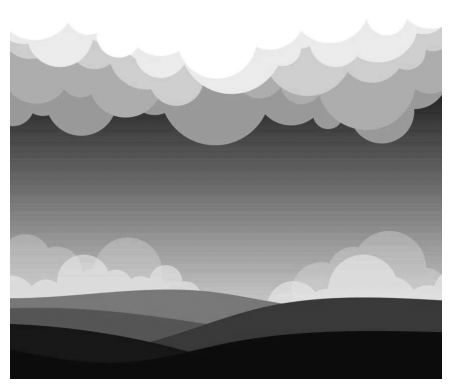
\includegraphics[width=0.5\textwidth]{cpu_processed.png}
    \caption{CPU Grayscale image}
    \label{fig:cpu_processed}
\end{figure}

\section{CUDA GPU Implementation}

The second implementation uses CUDA through the Numba library to accelerate the grayscale conversion on the GPU. Unlike the CPU implementation, which processes pixels sequentially, the GPU implementation distributes the computation across multiple CUDA threads, allowing many pixels to be processed simultaneously. For the same test image, the CUDA implementation completed the grayscale conversion in approximately 0.094863 seconds, which demonstrates the significant reduction in processing time achieved through parallel GPU execution.
\begin{figure}[H]
    \centering
    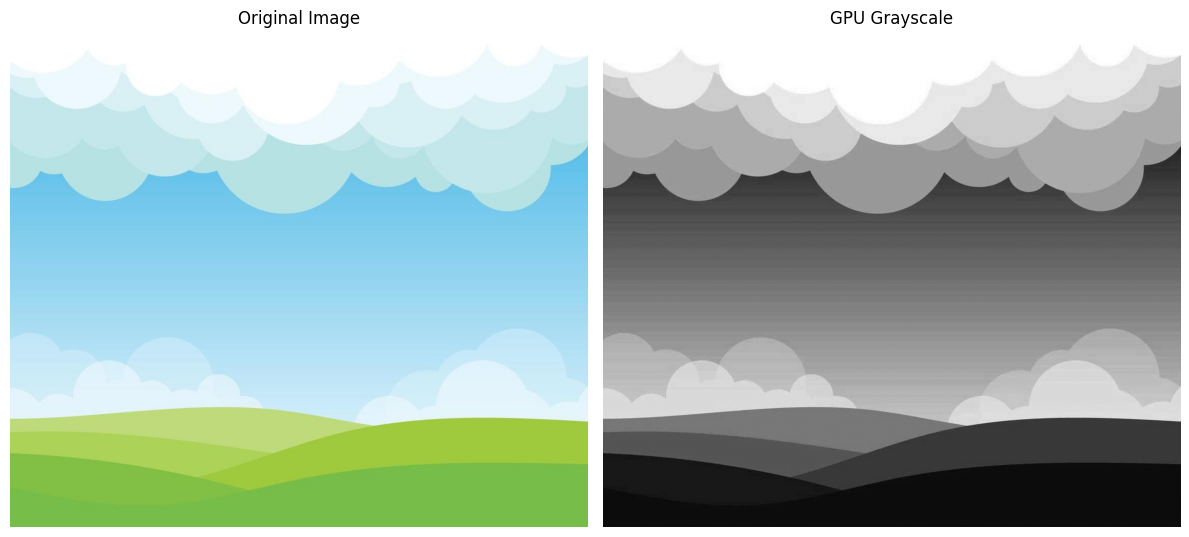
\includegraphics[width=0.9\textwidth]{gpu_processed.png}
    \caption{GPU}
    \label{fig:GPU_processed}
\end{figure}


\end{document}